% !TEX root = ../main.tex

\section{Introduction}
Self-driving is one of today's most impactful technological challenges, one that promises to bring
safe and affordable  transportation everywhere. Tremendous improvements have been made
in self-driving perception systems, thanks to the success of deep learning. This has enabled
accurate detection and localization of obstacles, providing a holistic understanding of the
surrounding world, which is then sent to the motion planner to decide subsequent driving actions.

Despite the eminent success of these perception systems, their detection
objective is \textit{mis-aligned} with the self-driving vehicle's overall goal---to drive
safely to the destination. We typically train the perception systems to detect all objects in
the sensor range, assigning each object an equal weight even if some objects are not important
as they will never interact with the self-driving vehicle. For example, they could be far away or
parked on the other side of the road as in Figure~\ref{fig:toy}.
As a result, a vast amount of computation and model capacity is wasted in recognizing
very difficult instances that matter only for common metrics such as average precision (AP), but not
so much for driving.
This is in
striking contrast with how humans drive: we focus our visual attention in areas that directly impact
safe planning. 
Inspired by the use of visual attention in our brain, we aim to introduce attention to self-driving systems to efficiently and selectively process complex scenes.

Numerous studies in the past have explored adding sparse attention in deep neural networks to
improve computation efficiency in  classification~\cite{resattn,adaptivecomp} and object
detection~\cite{sbnet,progressivesparse,recattend}. 
In order to perform well on the metrics employed in common benchmarks, the
attention mask in~\cite{sbnet} still needs to cover all actors in the scene, slowing the network when the scene has many vehicles.

In this paper, our aim is to address these inconsistencies such that the amount of computation is optimized towards the end goal of motion planning.
Specifically
our contributions are as follows:
\begin{itemize}
\item We learn an attention mask directly towards the motion planning objective for safe self-driving.
\item We use the attention mask to reweight object detection and motion forecasting losses in our
joint end-to-end training, focusing the model capacity on objects that matter most.
Different from manually prioritizing instances~\cite{prioritize}, here the weighting is entirely
data-driven.
\item Our attention-based model significantly reduced the
collision rate and improved planning performance while at a
much lower computation cost.
\item Attention mask visualization improves interpretability of end-to-end deep learning
models in self-driving.
\end{itemize}

\begin{figure}[t]
  \centering
  \iflatexml
  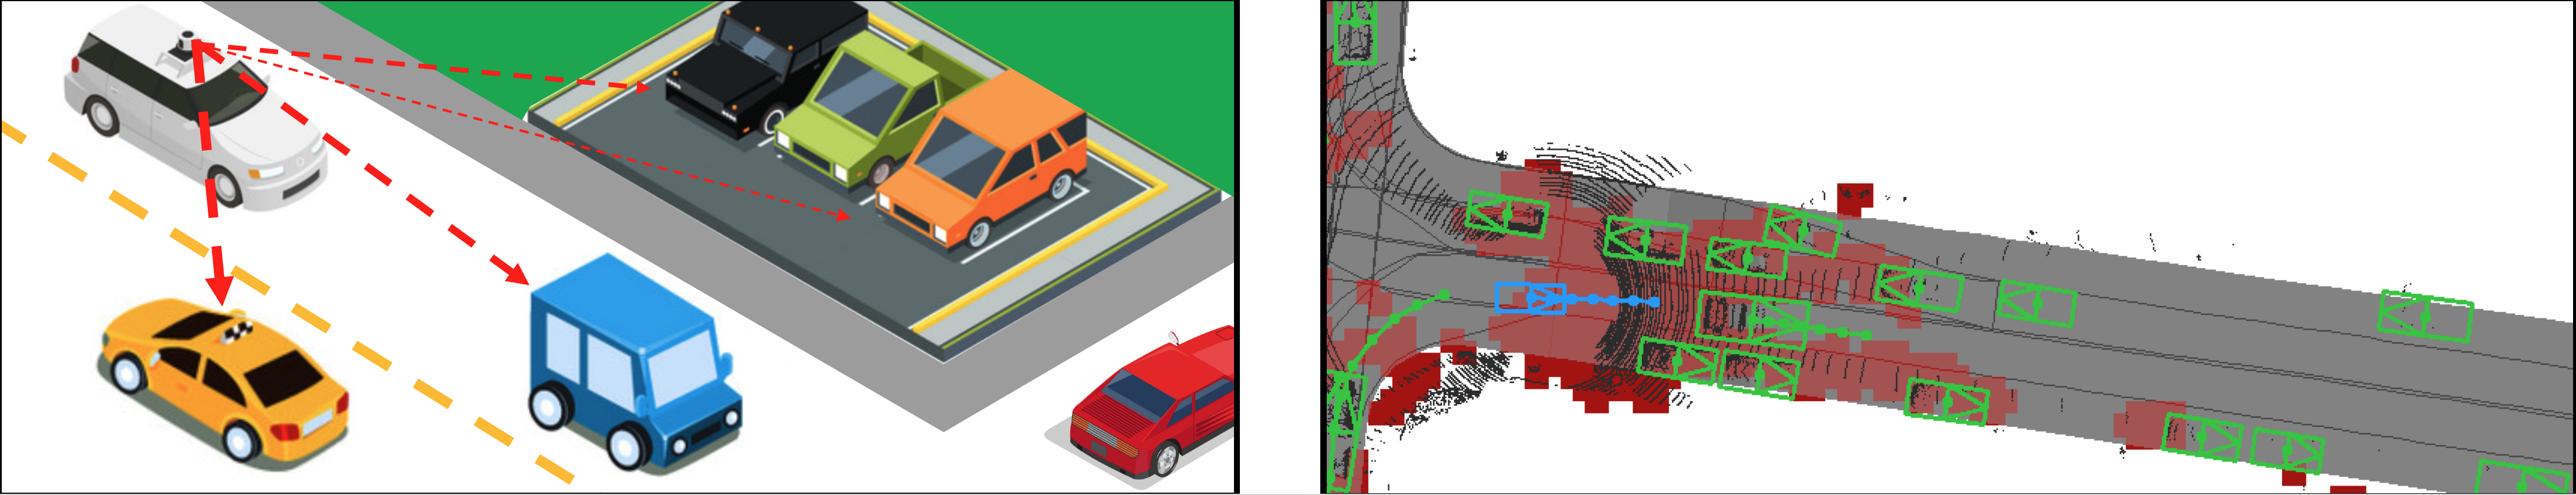
\includegraphics[width=6\textwidth]{figures/intro_vis.png}
  \else
  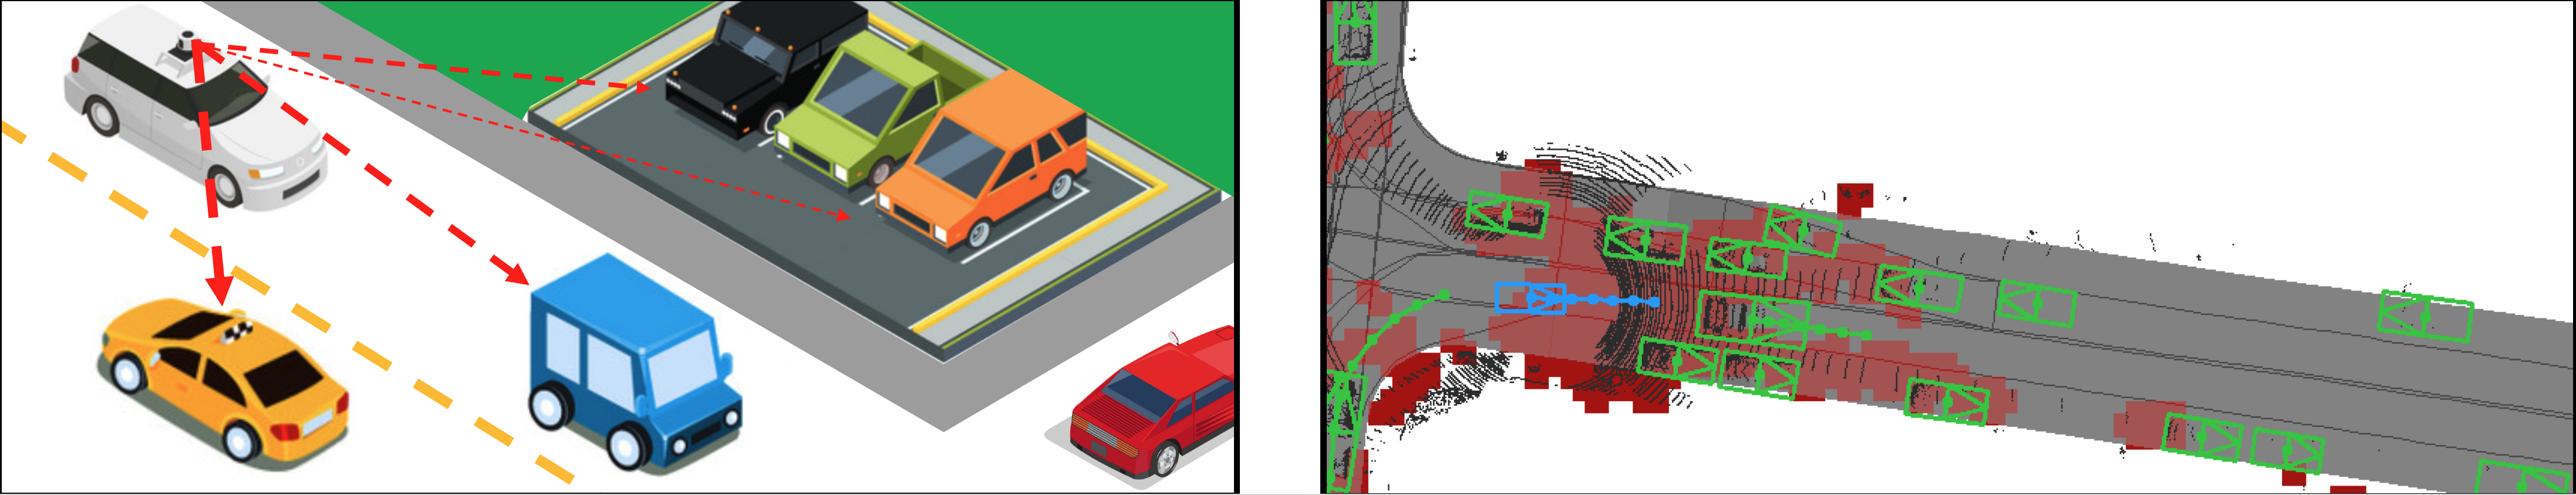
\includegraphics[width=\linewidth]{figures/intro_vis.pdf}
  \fi
  \caption{\small \textit{Left:} a toy example. \textit{Right:} our learned spatial attention in red with ego vehicle in blue and others in green. Not all actors impact our safe driving and so we should prioritize accordingly.}
  \label{fig:toy}
  \vspace{-0.15in}
\end{figure}